\documentclass{beamer}  
\mode<presentation>

%\usetheme{Singapore}
\usecolortheme{lily}
\usefonttheme[onlylarge]{structurebold}
\setbeamerfont*{frametitle}{size=\normalsize,series=\bfseries}
\setbeamertemplate{navigation symbols}{}
\setbeamercolor{frametitle}{bg=}
\setbeamercolor{titlelike}{parent=structure}

\definecolor{VitoBlue}{RGB}{83,163,220}
\definecolor{VitoOrange}{RGB}{245,130,32}
\definecolor{VitoGreen}{RGB}{103,175,62}
\definecolor{DarkBlue}{RGB}{0,46,86}
%\setbeamercolor{structure}{fg=VitoBlue}
%\setbeamercolor{normal text}{fg=DarkBlue}

\setbeamertemplate{blocks}[rounded][shadow=false]
%% \setbeamercolor{block title}{fg=VitoBlue}
%% \setbeamercolor{block title alerted}{fg=VitoBlue}
%% \setbeamercolor{block title example}{bg=blue!10,fg=VitoBlue}
%% \setbeamercolor{block body example}{bg=blue!5,fg=black!90}
%% \setbeamercolor{framesubtitle}{fg=VitoBlue}
%% \setbeamercolor{frametitle}{fg=VitoBlue}
%% \setbeamercolor{frametitle right}{fg=VitoBlue}
%% \setbeamercolor{title in head/foot}{fg=VitoBlue}
%% \setbeamercolor{title in sidebar}{fg=VitoBlue}
%% \setbeamercolor{titlegraphic}{fg=VitoBlue}
%% \setbeamercolor{titlelike}{fg=VitoBlue}

\setbeamertemplate{frametitle}
{
\begin{beamercolorbox}[wd=0.7\paperwidth]{frametitle}
  \insertframetitle
\end{beamercolorbox}
}
\usepackage{amsmath}
\usepackage{graphicx}
\usepackage{url}
\usepackage[overlay,absolute]{textpos}
\usepackage{tikz}
\usepackage{listings}
\usepackage{subfig}       % allows subfigures in single fig env
\usepackage{longtable} 
\usepackage{caption}
%\usepackage[pdftex]{color}

\def\myinline{\lstinline[basicstyle=\small\ttfamily,keywordstyle={}]}
\lstset{ %
%  backgroundcolor=\color{white},   % choose the background color; you must add \usepackage{color} or \usepackage{xcolor}
  basicstyle=\footnotesize\ttfamily,
%  basicstyle=\small,        % the size of the fonts that are used for the code
  breakatwhitespace=false,         % sets if automatic breaks should only happen at whitespace
  breaklines=true,                 % sets automatic line breaking
}

\def\postbreak{\raisebox{0ex}[0ex][0ex]{\ensuremath{\hookrightarrow\space}}}

\lstset{postbreak={\textbf{marker}\\space\\space\\space\\space}}
%\lstset{prebreak=\raisebox{0ex}[0ex][0ex]
%        {\ensuremath{\rhookswarrow}}}
\lstset{postbreak=\raisebox{0ex}[0ex][0ex]
        {\ensuremath{\hookrightarrow\space}}}
\lstset{breaklines=true, breakatwhitespace=true}

\newcommand\optionlabel[1]{\hspace{\labelsep}\textbf{\texttt{#1}}}
\newenvironment{option}
{%
   \let\descriptionlabel\optionlabel
   \description
   \setlength{\labelsep}{\textwidth}
}
{%
   \enddescription
}

\newcommand\optionlabelnb[1]{\hspace{\labelsep}\texttt{#1}}
\newenvironment{optionnb}
{%
   \let\descriptionlabel\optionlabelnb
   \description
   \setlength{\labelsep}{\textwidth}
}
{%
   \enddescription
}

\newcommand{\gdallogo}{
  \setlength{\TPHorizModule}{1pt}
  \setlength{\TPVertModule}{1pt}
   % textblock{}{x,y}: pos(x) = leftUpperCorner + (x * \TPHorizModule), pos(y) = leftUpperCorner - (y * \TPVertModule)
  \begin{textblock}{1}(330,220)
   \includegraphics[scale=0.15]{figures/logo_gdal}
  \end{textblock}
} 

\newcommand{\orfeologo}{
  \setlength{\TPHorizModule}{1pt}
  \setlength{\TPVertModule}{1pt}
   % textblock{}{x,y}: pos(x) = leftUpperCorner + (x * \TPHorizModule), pos(y) = leftUpperCorner - (y * \TPVertModule)
  \begin{textblock}{1}(330,220)
   \includegraphics[scale=0.2]{figures/logo_orfeo}
  \end{textblock}
} 

\newcommand{\pktoolslogo}{
  \setlength{\TPHorizModule}{1pt}
  \setlength{\TPVertModule}{1pt}
   % textblock{}{x,y}: pos(x) = leftUpperCorner + (x * \TPHorizModule), pos(y) = leftUpperCorner - (y * \TPVertModule)
  \begin{textblock}{1}(330,220)
   \includegraphics[scale=0.1]{figures/logo_pktools}
  \end{textblock}
} 

\newcommand{\rlogo}{
  \setlength{\TPHorizModule}{1pt}
  \setlength{\TPVertModule}{1pt}
   % textblock{}{x,y}: pos(x) = leftUpperCorner + (x * \TPHorizModule), pos(y) = leftUpperCorner - (y * \TPVertModule)
  \begin{textblock}{1}(330,220)
   \includegraphics[scale=1.0]{figures/logo_r}
%   \includegraphics[width=0.1\columnwidth]{figures/logo_r}
  \end{textblock}
} 


\setbeamertemplate{footline}{
%   \vitologo
   \begin{beamercolorbox}[ht=4ex,leftskip=1.4cm,rightskip=.3cm]{author in head/foot}
    \usebeamercolor{UniBlue}
    \hrule
    \vspace{0.1cm}
    \insertdate \hfill \inserttitle \newline
    %\insertshortauthor \ - \insertshortinstitute \hfill \insertframenumber
   \end{beamercolorbox}
   \vspace*{0.1cm}
} 

\newenvironment<>{varblock}[2][.9\textwidth]{%
  \setlength{\textwidth}{#1}
  \begin{actionenv}#3%
    \def\insertblocktitle{#2}%
    \par%
    \usebeamertemplate{block begin}}
  {\par%
    \usebeamertemplate{block end}%
  \end{actionenv}}

\title{Resource Planning Training Workshop - R-Statistics}
\subtitle{Coillte Forest (Limerick)}

\author{Daniel McInerney, Kevin O'Brien}

\date{}
 
\begin{document} 

\begin{frame}
\titlepage
\end{frame}

%\begin{frame}
%\frametitle{Content}
%\tableofcontents
%\end{frame}

%\addtobeamertemplate{frametitle}{}{%
%% \begin{tikzpicture}[remember picture,overlay]
%% \node[anchor=north east,yshift=-2pt] at (current page.north east) {\includegraphics[height=0.8cm]{figures/vito_basislogo}};
%% \end{tikzpicture}
\captionsetup[figure]{labelformat=empty}% redefines the caption setup of the figures environment in the beamer class.
%\setbeamertemplate{caption}{\insertcaption}

\section{Workshop Overview} 



\subsection{Workshop Series}
\begin{frame}
\frametitle{Resource Planning - Workshop Series}


\begin{table}[]
\begin{tabular}{lll}
Date 		& Training  	& Trainers  \\
\hline
19th Feb. 	& R Statistics  & dmci/kob   \\
26th Feb. 	& Python 1  	& jpp   \\
5th March 	& Python 2 	& jpp \\
12th March	& EO Data Processing & dmci \\
\hline
\end{tabular}
\end{table}

\end{frame}

\begin{frame}
\frametitle{Resource Planning - Workshop Structure}
\begin{itemize}
	\item Introduction to topics using hands-on exercises
	\item 10h00 to 16h00
	\item Breaks at 11.30, 13.00 and 15.30
\end{itemize}
\end{frame}


\section{R Primer} 



\subsection{Introduction to R}

 	%==============================================================================================%
	\begin{frame}
	\frametitle{Objectives of Workshop}
	\begin{itemize}
		\item Provide an introduction to the R Language
		\item Packages \& Task-Views
		\item Briefly explain data types
		\item Demonstrate how to read and write data
		\item Manipulating data
	\end{itemize}
	\end{frame}

 	%==============================================================================================%
 	\begin{frame}[fragile]
 		% % SLIDE 1 - COVER SLIDE
 		\begin{figure}
 			\centering
 			
\includegraphics[width=0.9\linewidth]{./figures/R_logo}
 		\end{figure}
 		\[ \mbox{Introduction to R} \]	
 	\end{frame}
 	

 	
 	%============================================================================= %

	\begin{frame}
	\frametitle{What is R?}
	\begin{itemize}
		\item R is a dialect of the S language (S-Plus)
		\item It follows S in terms of its linkage between graphics and data analysis
		\item It was initially written by Robert Gentleman and Ross Ihaka, who defined it as:
		\item "R is a language and environment for statistical computing and graphics"
		\item It is a programming environment within which statistical analysis  and visualisation is conducted.
		\item R has an extensive library of packages that offer state-of-the-art capabilities
	\end{itemize}
	\end{frame}


 	%==============================================================================================%
 	\begin{frame}
	\frametitle{R as a programming environment}
 		
 		\begin{itemize}
 			\item uses a well-developed but simple programming language
 			\item allows for rapid development of new tools according to user demand
 			\item these tools are distributed as packages, which any user can download to customize the R
 			environment.
 		\end{itemize}
 	\end{frame}
 	
 	%==============================================================================================%
 	\begin{frame}
 		\frametitle{Comprehensive R Archive Network}
 		\begin{itemize}
 			\item Base R and most R packages are available for download from the Comprehensive R Archive Network
 			(CRAN) cran.r-project.org. 
 			\item Base R comes with a number of basic data management,
 			analysis, and graphical tools 
 			\item R’s power and flexibility, however, lie in its array of packages
 			(currently more than 6,000!)
 		\end{itemize}
 		
 	\end{frame}
 	%==============================================================================================%


	\begin{frame}
	\frametitle{R-project Resources}
	\begin{block}{R Website}
	\begin{itemize}
		\item \url{http://r-project.org}
	\end{itemize}
	\end{block}
	\end{frame}

 	\begin{frame}
 		\frametitle{Comprehensive R Archive Network}
 		\begin{itemize}
 			\item Base R and most R packages are available for download from the Comprehensive R Archive Network
 			(CRAN) cran.r-project.org. 
 			\item Base R comes with a number of basic data management,
 			analysis, and graphical tools 
 			\item R’s power and flexibility, however, lie in its array of packages
 			(currently more than 6,000!)
 		\end{itemize}
 		
 	\end{frame}

	\begin{frame}
	\begin{block}{R Contributed Packages}
	\begin{itemize}
		\item \url{http://cran.r-project.org/web/packages/}
	\end{itemize}
	\end{block}
	\begin{block}{R Task View}
	\begin{itemize}
		\item \url{http://cran.r-project.org/web/views/}
		\item \url{http://cran.r-project.org/web/views/Spatial.html}
	\end{itemize}
	\end{block}
	\end{frame}

	\begin{frame}
	\frametitle{Some Important R Packages}

	\begin{block}{\texttt{dplyr}}
	A fast, consistent tool for working with data frame like objects,
	both in memory and out of memory.
	\end{block}

	\begin{block}{\texttt{ggplot2}}
	The ggplot2 package, created by Hadley Wickham, offers a powerful graphics language for creating elegant and complex plots. Its popularity in the R community has exploded in recent years. Origianlly based on Leland Wilkinson's The Grammar of Graphics, ggplot2 allows you to create graphs that represent both univariate and multivariate numerical and categorical data in a straightforward manner. Grouping can be represented by color, symbol, size, and transparency. The creation of trellis plots (i.e., conditioning) is relatively simple. 
	\end{block}
	\end{frame}

	\begin{frame}
	\frametitle{Some Important R-Spatial Packages}

	\begin{block}{\texttt{rgdal}}
	Provides bindings to Frank Warmerdam's Geospatial Data Abstraction Library (GDAL) (starting from 1.6.3, < 2) and access to projection/transformation operations from the PROJ.4 library. The GDAL and PROJ.4 libraries are external to the package, and, when installing the package from source, must be correctly installed first. Both GDAL raster and OGR vector map data can be imported into R, and GDAL raster data and OGR vector data exported. 
	\end{block}

	\begin{block}{\texttt{raster: Geographic data analysis and modeling}}
	Reading, writing, manipulating, analyzing and modeling of gridded spatial data. The package implements basic and high-level functions. Processing of very large files is supported.
	\end{block}
	\end{frame}
	%
	\begin{frame}
	\frametitle{Some Important R-Spatial Packages}

	\begin{block}{\texttt{sp: classes and methods for spatial data}}
	A package that provides classes and methods for spatial data. The classes document where the spatial location information resides, for 2D or 3D data. Utility functions are provided, e.g. for plotting data as maps, spatial selection, as well as methods for retrieving coordinates, for subsetting, print, summary, etc.
	\end{block}

	\begin{block}{\texttt{RColorBrewer: ColorBrewer Palettes}}
	Provides color schemes for maps and other graphics designed by Cynthia Brewer as described at %http://colorbrewer2.org
	\end{block}

	\end{frame}


\section{R Primer} 



\subsection{Installation}

 	%==============================================================================================%
	\begin{frame}
		\frametitle{R Installation}
	\begin{itemize}
		\item R is available as binaries \& source code for Windows, Mac and Linux
		\item \url{https://ftp.heanet.ie/mirrors/cran.r-project.org/}
	\end{itemize}
	However, R is also packaged within Rstudio
	\begin{itemize}
		\item open-source, IDE for R
		\item very user-friendly
		\item https://www.rstudio.com/products/rstudio/download/
	\end{itemize}
	\end{frame}

 	%==============================================================================================%
 	\begin{frame}[fragile]
	\frametitle{Let's spend some time checking our installation}
 		% % SLIDE 1 - COVER SLIDE
		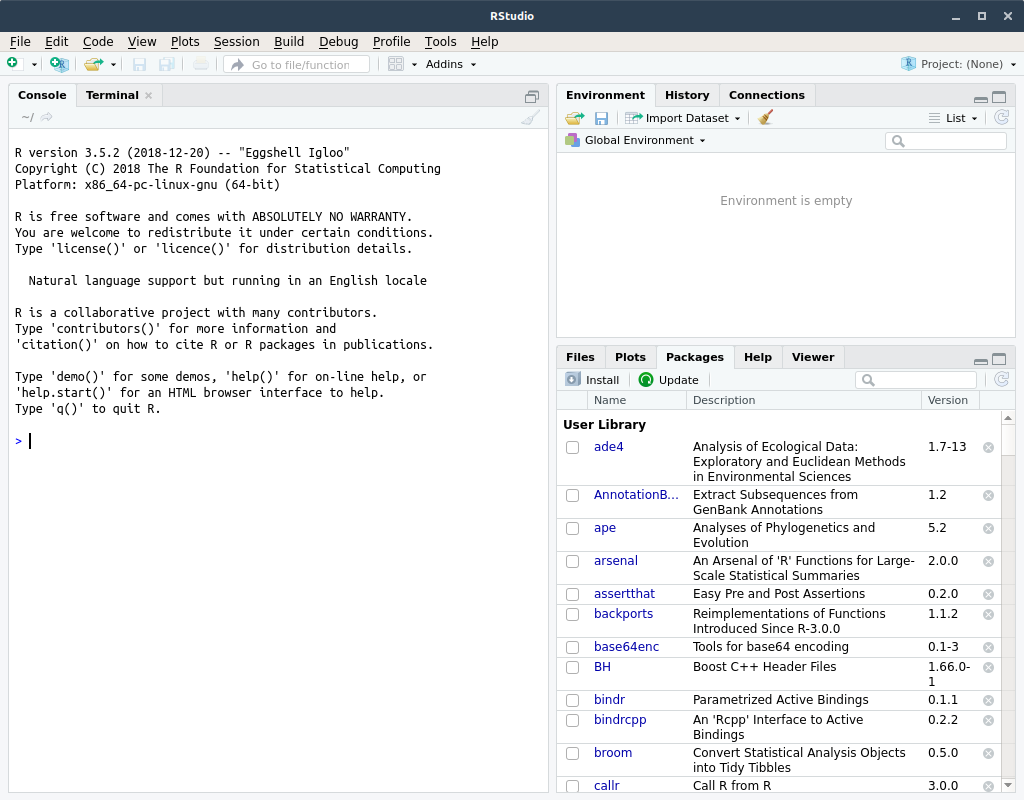
\includegraphics[scale=0.2]{./figures/rstudio}
 	\end{frame}
 	

 	


\end{document}
